\documentclass{beamer}

\usepackage{amssymb,amsmath}
\usepackage{calc}
%\usepackage{kbordermatrix}
\usepackage{booktabs}
\usepackage[absolute,overlay]{textpos}

%% ====== packages ==
\usepackage{style-article/police-speciale-bouquin}
\usepackage{style-article/enumeration-bouquin}
\usepackage{style-article/commande-hk-bouquin}
\usepackage{style-article/mathematique-bouquin}
\usepackage{ifthen} % pour commande-hk-bouquin
\usepackage{graphicx}
\usepackage{xspace}

% !! pour le francais
\usepackage[utf8]{inputenc}
\usepackage[T1]{fontenc}
%\usepackage[cyr]{aeguill}
\usepackage[francais]{babel}

%% ====== more def ==

\newcommand{\fleche}{\alert{$\pmb{\longrightarrow}$}~}
\newcommand{\flechenoire}{$\longrightarrow$~}
\renewcommand{\succeq}{\succcurlyeq}
\renewcommand{\preceq}{\preccurlyeq}
\newtheorem{proposition}{Proposition}
\newtheorem{defi}{Definition}
\newtheorem{theoreme}{Theorem}

%\newcommand{\E}{\mathbb{E}}
%\newcommand{\R}{\mathbb{R}}
%
%\newcommand{\aA}{\mathcal{A}}
%\newcommand{\CC}{\mathcal{C}}
%\newcommand{\FF}{\mathcal{F}}
%\newcommand{\EE}{\mathcal{E}}
%\newcommand{\II}{\mathcal{I}}
%\newcommand{\KK}{\mathcal{K}}
%\newcommand{\NN}{\mathcal{N}}
%\newcommand{\PP}{\mathcal{P}}
%\newcommand{\RR}{\mathcal{R}}
%\newcommand{\sS}{\mathcal{S}}

\newcommand{\kron}{\otimes}
\newcommand{\bbm}{\begin{bmatrix}}
\newcommand{\ebm}{\end{bmatrix}}
\newcommand{\ip}[2]{\langle #1, #2 \rangle}
\newcommand{\set}[1]{\left\{ #1 \right\}}
\newcommand{\sbr}[1]{\left[ #1 \right]}
\newcommand{\rbr}[1]{\left( #1 \right)}

%% ====== my bearmer ==
%\mode<presentation> {
%\usetheme{default}
%}
%
%% ** Headline:
%%\useoutertheme{miniframes}
%%\setbeamertemplate{headline}[miniframes theme]
%%\useoutertheme{infolines}
%%\setbeamertemplate{headline}[infolines theme]
%% Only show section name:
%\setbeamertemplate{headline}
%{%
%%\begin{beamercolorbox}{section in head/foot}
%\vskip2pt
%\hfill
%\insertsection
%\kern1em\vskip2pt
%%\end{beamercolorbox}%
%}
%
%% ** Frame titles:
%\setbeamerfont{frametitle}{size=\large}
%
%% ** Footline:
%%\setbeamertemplate{footline}[frame number]
%%\setbeamertemplate{footline}[text line]{\insertpagenumber}
%\setbeamertemplate{footline}
%{%
% \hfill%
% \usebeamercolor[fg]{page number in head/foot}%
% \usebeamerfont{page number in head/foot}%
% \insertpagenumber
% %\,/\,\insertpresentationendpage
% \kern1em\vskip2pt%
%}
%
%% ** Remove useless navigation symbols:
%\setbeamertemplate{navigation symbols}{}
%
%
%% options
%\useinnertheme[shadow]{rounded}  % les numeros
%\usefonttheme{structurebold}


\mode<presentation>
{
  \usetheme{Boadilla}
  %\usetheme{Madrid}
  %\usetheme{Warsaw}
  %\useinnertheme{default}
  
  %\usecolortheme{beaver}
  
%  albatross crane beetle
%  fly wolverine beaver

% Inner themes:
%  lily orchid rose

% Outer themes:
%  whale seahorse dolphin


%  \setbeamercovered{transparent}
}


\usenavigationsymbolstemplate{}

% Show the table of contents at the beginning of each sections
\AtBeginSection[]{
        \frame<beamer>{
\frametitle{Outline} \tableofcontents[current,currentsubsection]
  }}

\definecolor{orangeclair}{rgb}{1,0.92,0.83}
%\definecolor{mygrey}{rgb}{0.9,0.1,0.9} %  pas gris!
\definecolor{mygray}{gray}{0.6}

%% claude's def
\definecolor{blanc}{gray}{1}
\def\invisible#1{{\color{blanc}#1}}
\definecolor{brun}{rgb}{0.5,0.1,0.0}
\def\bistre#1{{\color{brun}#1}}
\def\bleu#1{{\color{blue}#1}}
\def\bleuclair#1{{\color{cyan}#1}}
\definecolor{gris}{gray}{0.5}
\def\explic#1{{\color{gris}#1}}
\def\rouge#1{{\color{red}#1}}
\definecolor{fonce}{rgb}{0.1,0.7,0}
\def\vert#1{{\color{fonce}#1}}

\def\image#1#2{\vspace{#2}\centerline{\input{#1.pstex_t}}\vspace{#2}}

\newcommand{\struct}[1]{\textcolor{structure}{\textbf{#1}}}
\newcommand{\mycite}[1]{\textcolor{blue}{#1}}

\newcommand{\mltbiqcrunch}{\emph{\mbox{MLTBiqCrunch}}}
\newcommand{\biqcrunch}{\emph{\mbox{BiqCrunch}}}


%% ====== title ==
\title[MLTBiqCrunch]{Résolution exacte du problème du stable par une approche mixte semidéfinie et polyédrale}
\author[Gandouin Leclercq Roupin]{\alert{Yolène Gandouin}$^*$, \alert{Etienne Leclercq}$^*$, \alert{Fr\'ed\'eric Roupin}$^*$}
\institute[LIPN]{$^{*}$LIPN, UMR 7030, Universit\'e Paris 13, Sorbonne Paris Cit\'e}
\date[Lorient ROADEF 2018]{ROADEF, Lorient -- F\'evrier 2018}

%% ====== begin ==
\begin{document}



%****************************************************************
\begin{frame}
\titlepage
\end{frame}

%****************************************************************
\begin{frame}
\frametitle{Plan de la présentation}

\Large{
\begin{itemize}
\item[-] \bleu{Contexte : le solveur \biqcrunch}
\vspace{2mm}
\item[-] \bleu{Parallélisation de \biqcrunch}
\vspace{2mm}
\item[-] \bleu{Résultats expérimentaux : comparaison avec la version séquentielle}
\vspace{2mm}
\item[-] \bleu{Perspectives et développements futurs} 
\end{itemize}
}

\end{frame}

%****************************************************************
\begin{frame}
\frametitle{Présentation de \biqcrunch}

{\tiny
  \begin{thebibliography}
    \beamertemplatearticlebibitems
    
\bibitem{KMR:2016}
Nathan Krislock, Jerome Malick, et Fr{\'e}d{\'e}ric Roupin. (2016)
\newblock {Biqcrunch: a semidefinite branch-and-bound method for solving binary quadratic problems}.
ACM Transactions on Mathematical Software 43(4).
 
\end{thebibliography}
}

\begin{block}{example.lp}
\begin{small}
Maximize
20 z1*z3 + 26 z1*z4 + 23 z2*z3 + 8 z2*z5 + 32 z3*z4 + 13 z4*z5 

Subject to

  z1 + z2 + z3 + z4 + z5 = 3

  12 z1*z3 + 24 z1*z4 + 14 z2*z3 + 16 z2*z5 + 28 z3*z4 + 12 z4*z5 <= 30

Binary

  z1 z2 z3 z4 z5
  
End
\end{small}
\end{block}


\begin{itemize}
\item Le code, entièrement open-source, est disponible : 
\centers{\fcolorbox{black}{white}{www-lipn.univ-paris13.fr/BiqCrunch}}
\item Solveur exact (Branch-and-Bound) de \bleu{tout problème quadratique ou linéaire en variables 0-1}
\item Fondé sur une famille de relaxations dont la qualité est \bleu{ajustée dynamiquement} à chaque n\oe ud de l'arbre de recherche
\end{itemize}

\end{frame}

%****************************************************************
\begin{frame}
\frametitle{Présentation de \biqcrunch}

\begin{block}{Spécificités de \biqcrunch}
\begin{itemize}
\item Lors de l'évaluation de chaque n\oe ud les relaxations non-linéaires sont renforcées par des inégalités triangulaires
\item L'approche duale adoptée pour la résolution des relaxations permet d'interrompre l'évaluation à tout moment (bornes toujours valides)
\item Les temps d'évaluation sont bornés par un mécanisme de "give up" lorsqu'il est peu probable que le n\oe ud puisse être élagué.
\item \bleu{Très peu de mémoire} utilisée : quelques Mo pour un problème comportant plusieurs centaines de variables.
\item Dans sa version actuelle : BiqCrunch effectue \bleu{uniquement des calculs séquentiels (un seul thread)}
\end{itemize}
\end{block}

\begin{block}{\alert{Objectif :} proposer une version multithread}

Le bénéfice pour un algorithme de type Branch-and-Bound peut être important : possible speedup superlinéaire.
\end{block}

\end{frame}

%****************************************************************
\begin{frame}
\frametitle{Eléments constitutifs de \biqcrunch}

\begin{block}{Composants et bibliothèques}

\begin{itemize}
\item Utilisation importante de \bleu{fonctions BLAS et LAPACK} (en particulier décomposition spectrale de matrices)
\item L-BFGS-B : \bleu{méthode quasi-Newtonienne} utilisant également BLAS et LAPACK pour la résolution des relaxations non-linéaires
\item Une version modifiée du \bleu{framework BOB} qui permet :
\begin{itemize}
\item d'obtenir un code orienté performance
\item un \bleu{réglage simple} des stratégies de parcours, d'équilibrage, du choix des structures de données (file d'attente)
\item de définir complètement la fonction de \bleu{séparation} (par exemple fixation de plusieurs variables simultanément)
\item  un contrôle précis de la fonction d'\bleu{évaluation} (interruption précoce), et des heuristiques
\end{itemize}

\end{itemize}
\end{block}
\end{frame}


%****************************************************************
\begin{frame}
\frametitle{La parallélisation de \biqcrunch}

\begin{block}{Deux grains de parallélisation considérés}
\begin{itemize}
\item Pour le branch-and-bound : un thread par noeud (BOB)
\item Pour l'évaluation du noeud : paralléliser les appels à BLAS \fleche MLTBLAS
\item \alert{La granularité doit être contrôlée} sous peine de perte de performances
\end{itemize}
\end{block}

\begin{block}{Modifications principales apportées}
\begin{itemize}
\item Gestion de la mémoire partagée : chaque évaluation de n\oe ud possède sa propre zone de mémoire.
\item \alert{Ajout de deux paramètres supplémentaires} à BiqCrunch permettant de sélectionner :
\begin{itemize}
\item  le \bleu{nombre total de threads} à utiliser
\item  à chaque évaluation : le \bleu{ratio de threads disponibles} à utiliser par les routines BLAS parallèles 
\end{itemize}
\alert{\fleche} Permet de régler les deux niveaux de parallélisation
%\item Utilisation de la bibliothèque openBLAS
%\item Remplacement des appels BLAS et LAPACK dans L-BFGS-B (versions plus anciennes) pour une meilleure performance
\end{itemize}
\end{block}
\end{frame}

%----------------------------------------------------------

\begin{frame}
	\frametitle{Réglage des deux niveaux de parallélisation}

\begin{block}{Profil de performance}
\begin{small}
\[
	\theta(\tau) = \frac{1}{|\mathcal{P}|} \left| \set{ p \in \mathcal{P} : t_{p} \leq \tau t_{p}^{\min} } \right|, \quad \text{pour $\tau \geq 1$}
\]

\vspace{-7mm}
\begin{align*}
\mathcal{P} &= \ \text{Ensensemble de 45 instances du problème $k$-cluster $n=100$} \\
t_p &= \ \text{temps pour résoudre $p$ pour l'algorithme, } t_p^{\min}= \ \text{meilleur temps }
\end{align*}
\end{small}
\vspace{-7mm}
\end{block}

%=> FIGURE à insérer : 8 threads, MLTBlas dans {1,2,4,8}

\alert{Ici :} le niveau à privilégier est celui du n\oe ud. Résultats pour $8$ threads :

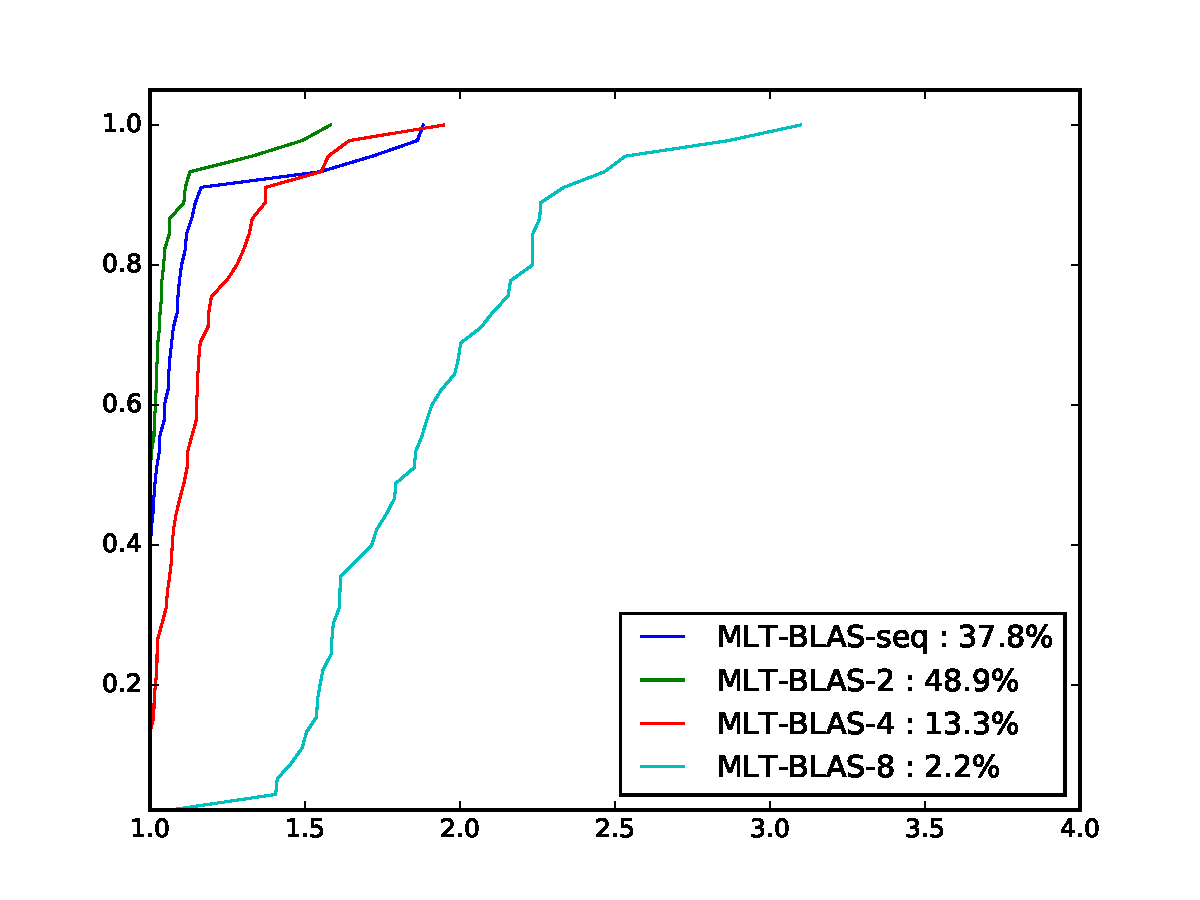
\includegraphics[scale=0.33]{fig/MLT-BLAS.pdf} 

\end{frame}


%****************************************************************
\begin{frame}
\frametitle{Problème $k$-cluster}

Soit $G=(V,E)$ dont les arêtes sont pondérées par une matrice $W$, et un entier $0<k<n$.

\centers{\fcolorbox{black}{white}{Trouver le sous-graphe de $k$ sommets de poids maximal}}

\begin{block}{Modélisation par un programme quadratique 0-1}

\[
\begin{tabular}{ll}
$(\text{KC})$ &
\fbox{
	\begin{tabular}{lll}
	maximiser 	& $\frac{1}{2} z^T W z$ \\
	sous contraintes 	& $\sum_{i=1}^n z_i = k$\\
				& $z \in \set{0,1}^n$
	\end{tabular}
}
\end{tabular}
\]

Pour $j \in \set{1,\ldots,n}$, on ajoute les contraintes redondantes $\sum_{i=1}^n z_i z_j = k z_j$ qui permettent de renforcer les relaxations sous-jacentes utilisées par le solveur

\end{block}


\end{frame}

%****************************************************************
\begin{frame}
\frametitle{Profils de performance pour le problème $k$-cluster}

\begin{block}{Comportement en fonction du nombre de threads}
\begin{itemize}
\item Ensemble de 45 instances du problème $k$-cluster 	avec $n=100$
\item Réglage de deux niveaux de parallélisation : MLT-BLAS utilise en général au plus $2$ threads
\item Le nombre total de threads varie de $1$ à $8$
\end{itemize}
\end{block}

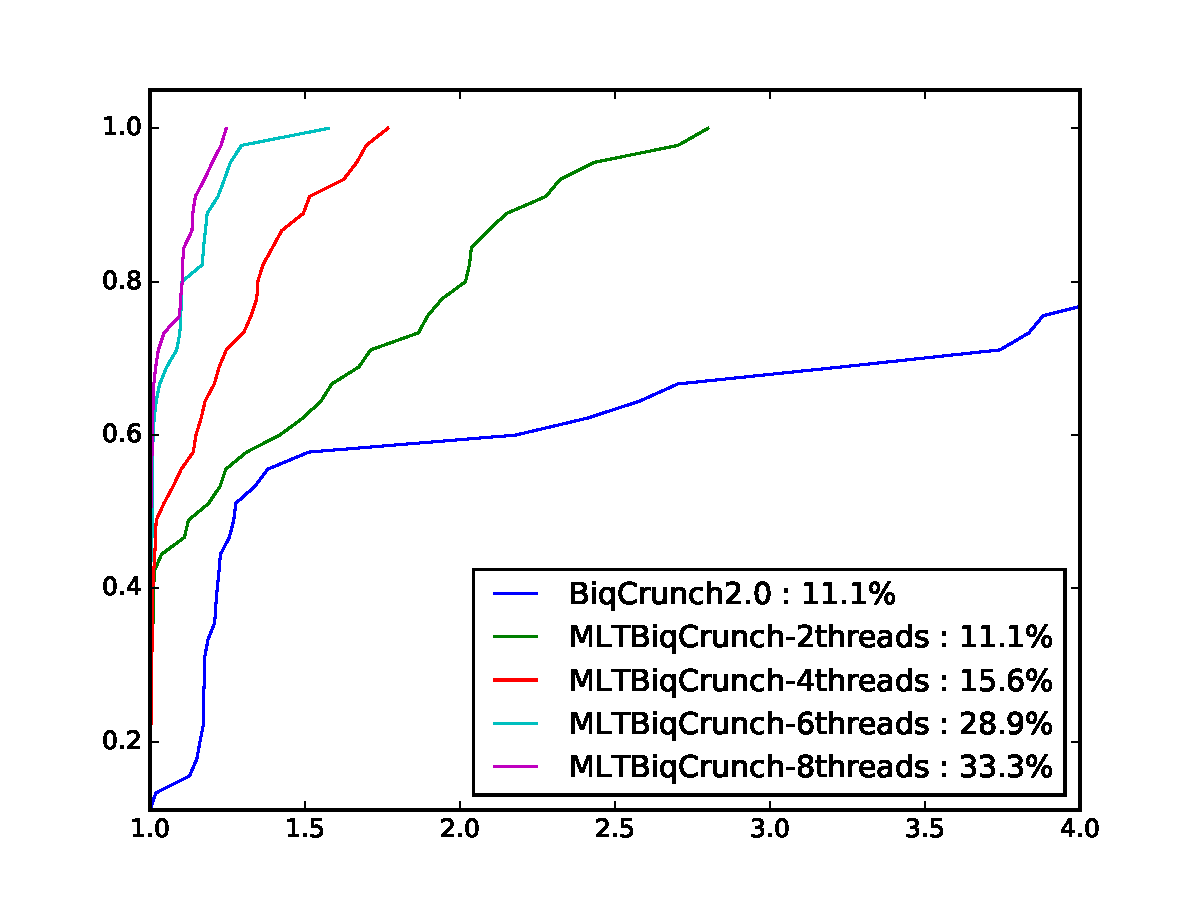
\includegraphics[scale=0.33]{fig/MLTBiqCrunch0.pdf}

\end{frame}

%----------------------------------------------------------

\begin{frame}
\frametitle{Résultats numériques pour $k$-cluster}

\begin{block}{Problèmes de taille $120$ : $5$ instances par ligne}

\begin{tabular}{ll}
{\scriptsize
\begin{tabular}{cccrr}
\multicolumn{3}{c}{\alert{BiqCrunch 2.0}} & & \\
\hline\noalign{\smallskip}
$n$ & $k$ & $d$(\%) & nodes & time (s) \\
\noalign{\smallskip}\hline\noalign{\smallskip}
120 & 30 & 25 & 64.6 & 133.04 \\
 & & 50 & 110.6 & 177.20 \\
 & & 75 & \textbf{236.6} & \textbf{297.84} \\
 & 60 & 25 & 28.6 & 59.09 \\
 & & 50 & 43.8 & 90.66 \\
 & & 75 & 19.0 & 38.95 \\
 & 90 & 25 & 1.0 & 3.53 \\
 & & 50 & 6.2 & 28.79 \\
 & & 75 & \textbf{1.0} & \textbf{2.38} \\
\noalign{\smallskip}\hline
\end{tabular}
}

&
{\scriptsize
\begin{tabular}{cccrr}
\multicolumn{3}{c}{\alert{MLTBiqCrunch}} & & \\
\hline\noalign{\smallskip}
$n$ & $k$ & $d$(\%) & nodes & time (s) \\
\noalign{\smallskip}\hline\noalign{\smallskip}
120 & 30 & 25 & 54.6 & 29.56 \\
 & & 50 & 109.0 & 43.73 \\
 & & 75 & \textbf{222.4} & \textbf{70.05} \\
 & 60 & 25 & 27.4 & 21.36 \\
 & & 50 & 43.0 & 28.41 \\
 & & 75 & 19.0 & 16.76 \\
 & 90 & 25 & 1.0 & 3.54 \\
 & & 50 & 7.4 & 20.05 \\
 & & 75 & \textbf{1.0} & \textbf{2.24} \\
\noalign{\smallskip}\hline
\end{tabular}
}
\end{tabular}
\end{block}

\begin{itemize}
\item Le nombre de threads utilisés vaut ici $4$
\item Lorsque le nombre de n\oe uds est faible, la parallélisation (BLAS) n'est pas rentable car les temps d'évaluation sont trop courts
\item On observe déjà pour certaines instances un speed-up superlinéaire
\end{itemize}

%{\tiny
%  \begin{thebibliography}
%    \beamertemplatearticlebibitems
%    
%\bibitem{Krislock:2012a}
%Nathan Krislock, Jerome Malick, et Fr{\'e}d{\'e}ric Roupin. (2016)
%\newblock {Computational results of a semidefinite branch-and-bound algorithm for $k$-cluster}.
%Computers and Operations Research, 66: 153-159.
% 
%\end{thebibliography}
%}


\end{frame}

%----------------------------------------------------------

\begin{frame}
\frametitle{Résultats numériques pour $k$-cluster}

\begin{block}{Problèmes de taille $160$ : $5$ instances par ligne}

\begin{tabular}{ll}
{\scriptsize
\begin{tabular}{cccrr}
\multicolumn{3}{c}{\alert{BiqCrunch 2.0}} & & \\
\hline\noalign{\smallskip}
$n$ & $k$ & $d$(\%) & nodes & time (s) \\
\noalign{\smallskip}\hline\noalign{\smallskip}
160 & 40 & 25 & 501.0 & 1927.53 \\
 & & 50 & 6061.6 & \textbf{15411.70} \\
 & & 75 & 4427.8 & 10798.50 \\
 & 80 & 25 & 207.4 & 854.28 \\
 & & 50 & 505.8 & 1791.06 \\
 & & 75 & 2017.4 & 7242.98 \\
 & 120 & 25 & 10.2 & 74.53 \\
 & & 50 & 7.0 & 63.67 \\
 & & 75 & 3.8 & 30.64 \\
\noalign{\smallskip}\hline
\end{tabular}
}
&
{\scriptsize
\begin{tabular}{cccrr}
\multicolumn{3}{c}{\alert{MLTBiqCrunch}} & & \\
\hline\noalign{\smallskip}
$n$ & $k$ & $d$(\%) & nodes & time (s) \\
\noalign{\smallskip}\hline\noalign{\smallskip}
160 & 40 & 25 & 535.4 & 397.59 \\
 & & 50 & 6430.6 & \textbf{3731.51} \\
 & & 75 & 5103.8 & 2624.43 \\
 & 80 & 25 & 195.4 & 177.25 \\
 & & 50 & 536.6 & 471.94 \\
 & & 75 & 2101.4 & 1786.57 \\
 & 120 & 25 & 10.6 & 38.75 \\
 & & 50 & 6.2 & 30.95 \\
 & & 75 & 5.0 & 28.39 \\
\noalign{\smallskip}\hline
\end{tabular}
}
\end{tabular}

\end{block}

\begin{itemize}
\item Le nombre de threads utilisés vaut ici $4$
\item Le nombre de n\oe uds évalués est du même ordre de grandeur
\item Les speed-up est linéaire voire superlinéaire en particulier pour les instances les plus difficiles
\end{itemize}

%{\tiny
%  \begin{thebibliography}
%    \beamertemplatearticlebibitems
%    
%\bibitem{Krislock:2012a}
%Nathan Krislock, Jerome Malick, et Fr{\'e}d{\'e}ric Roupin. (2016)
%\newblock {Computational results of a semidefinite branch-and-bound algorithm for $k$-cluster}.
%Computers and Operations Research, 66: 153-159.
% 
%\end{thebibliography}
%}


\end{frame}


%****************************************************************
\begin{frame}
\frametitle{Le Problème Max Stable}

Soit $G=(V,E)$ dont les sommets sont pondérés par un vecteur $w$.

\centers{\fcolorbox{black}{white}{Trouver le stable de $G$ de poids maximal}}

\begin{block}{Modélisation par un programme quadratique 0-1}

\[
\begin{tabular}{ll}
$(\text{MIS})$ &
\fbox{
	\begin{tabular}{lll}
	maximiser 	& $w^Tx$ \\
	sous contraintes 	& $x_ix_j = 0$, & $(i,j)\in E$\\
				& $x \in \set{0,1}^n$
	\end{tabular}
}
\end{tabular}
\]
\end{block}

\begin{block}{Problèmes de la bibliothèque DIMACS}

\begin{tabular}{ll}
{\scriptsize
\begin{tabular}{lccrr}
\multicolumn{3}{c}{\alert{BiqCrunch 2.0}} & & \\
\hline\noalign{\smallskip}
 & $n$ & $m$ & nodes & time (s) \\
\noalign{\smallskip}\hline\noalign{\smallskip}
MANN\_a9 & 45 & 72 & 5 & 3.90 \\
keller4 & 171 & 5100 & 155 & 155.24 \\
brock200\_1 & 200 & 5066 & 1393 & 1822.81 \\
brock200\_2 & 200 & 10024 & 53 & 87.01 \\
brock200\_3 & 200 & 7852 & 107 & 157.45 \\
brock200\_4 & 200 & 6811 & 185 & 263.32 \\
\noalign{\smallskip}\hline
\end{tabular}
}
&
{\scriptsize
\begin{tabular}{rr}
\multicolumn{2}{c}{\alert{MLTBiqCrunch}} \\
\hline\noalign{\smallskip}
 nodes & time (s) \\
\noalign{\smallskip}\hline\noalign{\smallskip}
 3 & 0.64 \\
 113 & 88.55 \\
 2861 & 747.38 \\
 79 & 73.78 \\
 321 & 113.04\\
 185 & 77.51 \\
\noalign{\smallskip}\hline
\end{tabular}
}
\end{tabular}

\end{block}

\end{frame}

%%****************************************************************
%\begin{frame}
%\frametitle{Résultats expérimentaux - $\pmb{k}$-cluster - $n=100$ et $n=120$}
%
%\end{frame}
%
%%****************************************************************
%\begin{frame}
%\frametitle{Résultats expérimentaux - $\pmb{k}$-cluster - $n=140$ et $n=140$}
%
%\end{frame}
%
%%****************************************************************
%\begin{frame}
%\frametitle{Résultats expérimentaux}
%
%\end{frame}

%****************************************************************
\begin{frame}
\frametitle{Perspectives et développements futurs}

\begin{itemize}

\item Gestion différente de la file d'attente (par exemple attente active/passive des threads)
\item \bleu{Equilibrage} entre BLAS et \mltbiqcrunch ~à reconsidérer pour des problèmes dont les \bleu{évaluations sont plus longues} (par exemple, l'affectation quadratique).
\item Les choix actuels ont été conduits pour une utilisation sur une \bleu{machine standard} ($4$ ou $8$ c\oe urs) à mémoire partagée : considérer des matériels / architectures \bleu{différents}.
\item Tester d'\bleu{autres fonctions de séparation} (arbres de recherche plus larges mais moins profonds).

\end{itemize}

\end{frame}

%****************************************************************
\begin{frame}

\includegraphics[scale=0.44]{fig/BiqHome.pdf}

\end{frame}


\end{document}
